\documentclass[sigplan,screen,10pt]{acmart}
\usepackage[utf8]{inputenc}
\usepackage[T1]{fontenc}
\usepackage[french]{babel}
\usepackage{xcolor}
\newif\ifshowcomments
\showcommentstrue

\ifshowcomments
%\newcommand{\mynote}[2]{\fbox{\bfseries\sffamily\scriptsize#1}
\newcommand{\mynote}[2]{\fbox{\bfseries\sffamily\footnotesize{\textbf{#1}}}
 {\small$\blacktriangleright$\textsf{\emph{#2}}$\blacktriangleleft$}}
\else
\newcommand{\mynote}[2]{}
\fi
\newcommand{\stella}[1]{\mynote{\textcolor{red}{Stella}}{\textcolor{blue}{\textbf{#1}}}}

\begin{document}
	\section*{Number of accesses per snapshot}
	
	Figures~\ref{fig:xxx} and~\ref{fig:xxx} describe, the average number of accesses to a snapshot during the workload.
	%This describe, the number of accesses to a same cluster per snapshot during a workload.
	We present the results for disk images of 50 and 500 snapshots.
%	I focus here on chain of 50 and 500 snapshots.
	We can observe that with vanilla, the number of accesses per snapshoht is much larger compared to direct-access \stella{il faut voir avec Alain la nomenclature à suivre tout au long du papier. Il va sûrement la définir dès l'intro et c'est la même que tu devras employer pour qu'on te suive dans la lecture du papier. que ce soit pour les noms des versions (vanilla, direct access) ou des disques (chain, image, disk image)}.
	This is explained by the fact that, to access a specific cluster, vanilla needs to access each cluster in all previous intermediate snapshots to find which one contains this cluster.
	%because we are always looking for all the pasts snapshots in order to find a specific cluster.
	In contrast, direct-access directly accesses the index of the snapshot that contains the target cluster.
	%With our direct-access method, we only have the exact number of accesses which give us the real index and then we can jump to that snapshot index, omitting access to intermediate snapshots.
	
	\begin{figure}[h]
		\center
		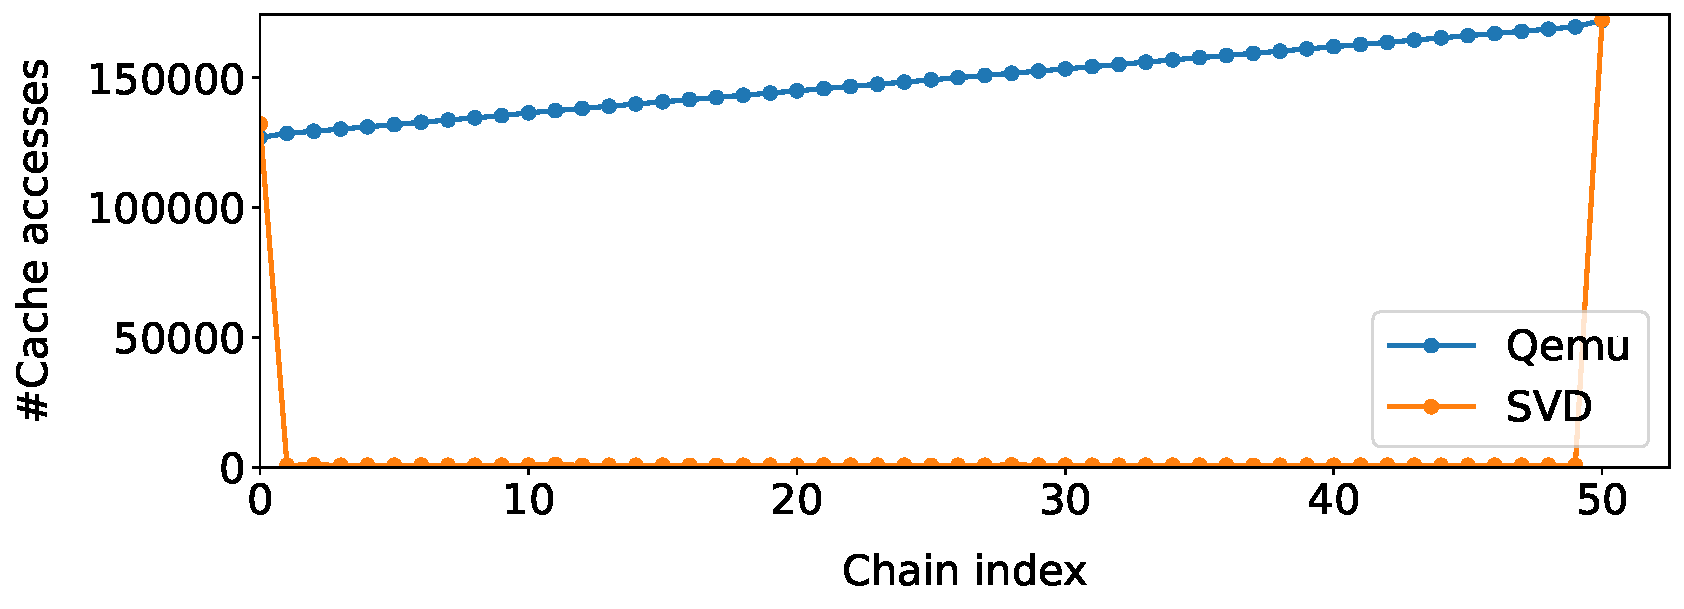
\includegraphics[width=0.45\textwidth]{clusters_accesses_chain_50.pdf}
		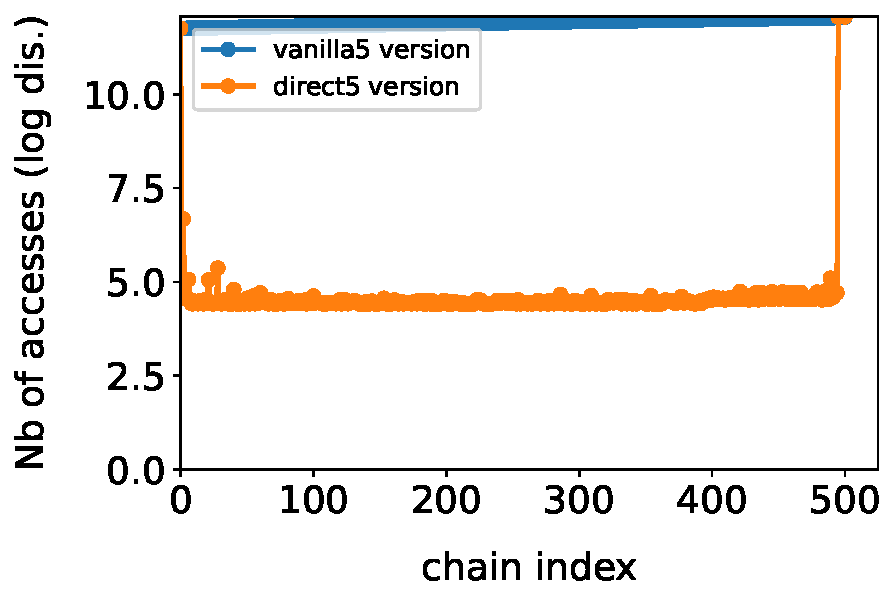
\includegraphics[width=0.45\textwidth]{clusters_accesses_chain_500.pdf}
		\caption{Accesses per sanspshots for a chain of 50 snapshots (on the left) and 500 snapshots (on the right).}
		\label{fig:fig2}
	\end{figure}


	\section*{Events when accessing a snapshot}% (events)
	Accessing a snapshot can results in one of the following events:
	% Here, we focus on explaining why there are more accesses in vanilla version, and we are doing it by distinguishing all the type of access results (here we call it \textit{event}) in each chain.
	\begin{itemize}
		\item normal => the cluster is allocated in the current snapshot (after we resolved an unallocated event ~\stella{ça veut dire quoi que le normal survient toujours après le "unallocated"? et quand on trouve donc directement le cluster c'est quoi l'évt dans ce cas?)}
		\item unallocated => the cluster is not allocated~\stella{allocated ou present? c'est quoi la diff?} in the current snapshot
		\item cache missed (\stella{je pense qu'il faudrait changer ça partout et appeler ça miss sans le "ed" car ce à quoi on est habitué et qui sonne normal comme tlb miss}) => the cluster metadata are or not in the cache
		\item cache hit => the cluster metadata are present in the cache
	\end{itemize}
		
	\begin{figure}[h]
		\center
		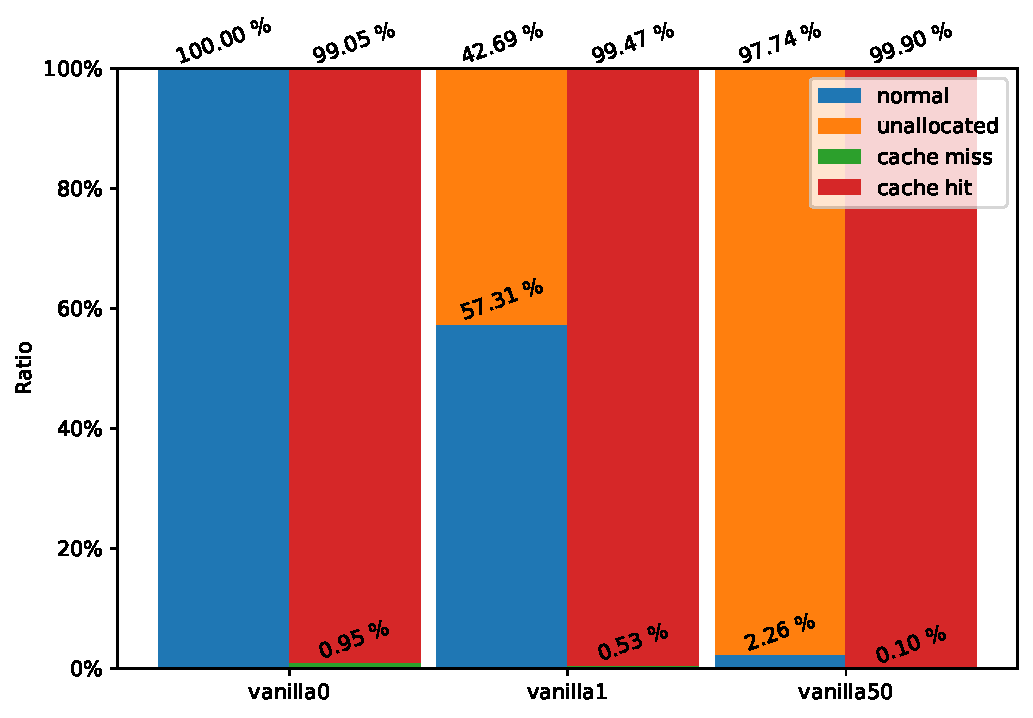
\includegraphics[width=0.6\textwidth]{number_events_per_chain_va.pdf}
		\caption{Number of events (unallocated, missed, hit, normal) with vanilla for chains of 0, 1, and 50 snapshots.\stella{je me dis que si tu voulais expliquer pq le nb d'accès avec vanilla (fig. précédente) alors ça aurait été bien de prendre les mm tailles de chaines}}
		\label{fig:fig36}
	\end{figure}

	We can observe that with vanilla, the number of unallocated to access a given cluster (i.e., to obtain a \emph{normal} event) increases exponentially with the numer of snapshots.
	While with direct-access, we almost always have the same number of \emph{unallocated} and \emph{normal} events regardless the number of snapshots.
	This is due to the fact that with direct-access, an \emph{unallocated} event is not propagated all over the chain but rather resloved in the snapshot where it occurs (\stella{qu'est ce que tu entends pas "propagated" on ne comprend pas. tu n'nas pas dit pour vanilla qu'on propageait l'évt donc un peu perdu}).
	% We noticed that in the vanilla version, the number of unallocated events that we get in order to get the current location of the cluster (normal event occurence) increased exponentially with the chain of the length. While in our direct-access version, we always approximatively have the same number of unallocated and normal event regardless of the chain length, this due to the fact that a same "unallocated event" is not propagate all over the chain like in the vanilla version.
	
	\begin{figure}[h]
		\center
		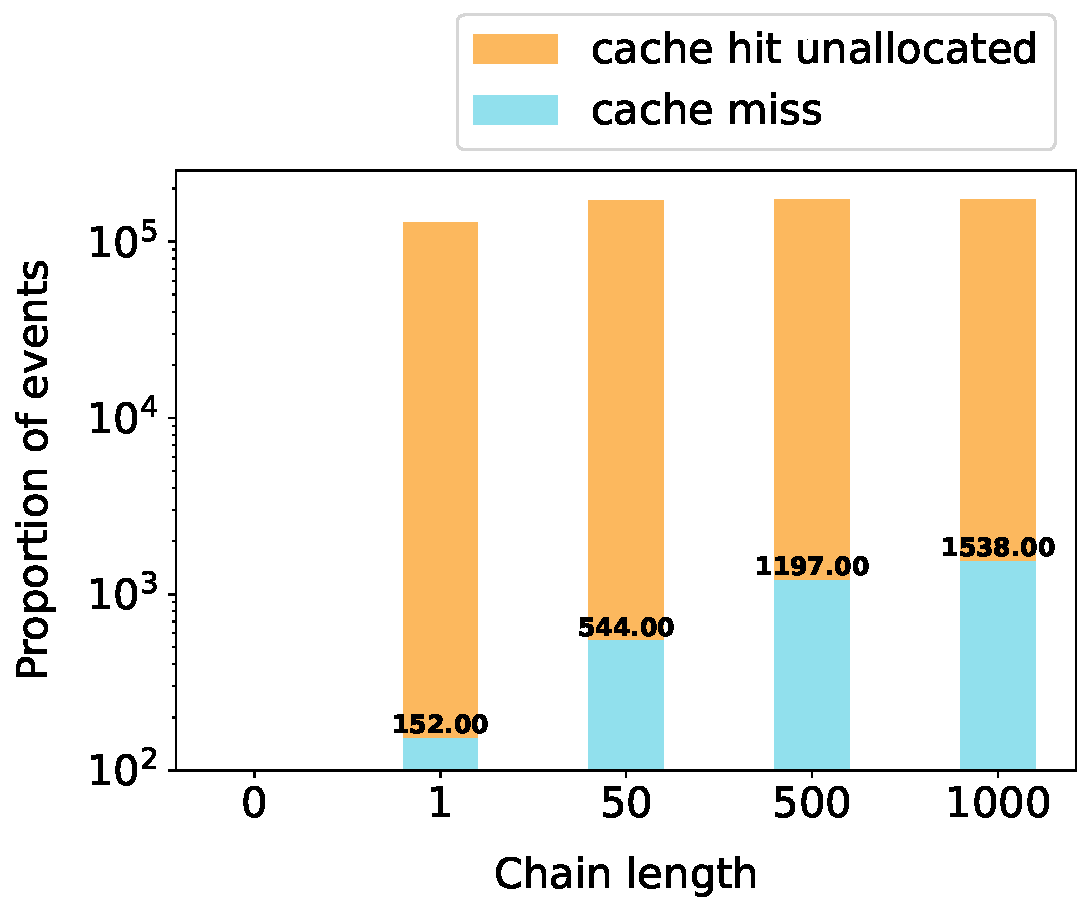
\includegraphics[width=0.6\textwidth]{number_events_per_chain_di.pdf}
		\caption{Number of events (unallocated, missed, hit, normal) with direct-access.}
		\label{fig:fig37}
	\end{figure}


	\section*{Memory footprint}
	
	Memory footprint and throughput comparison between vanilla and direct-access during dd workload.
	
	\begin{figure}[h]
		\center
		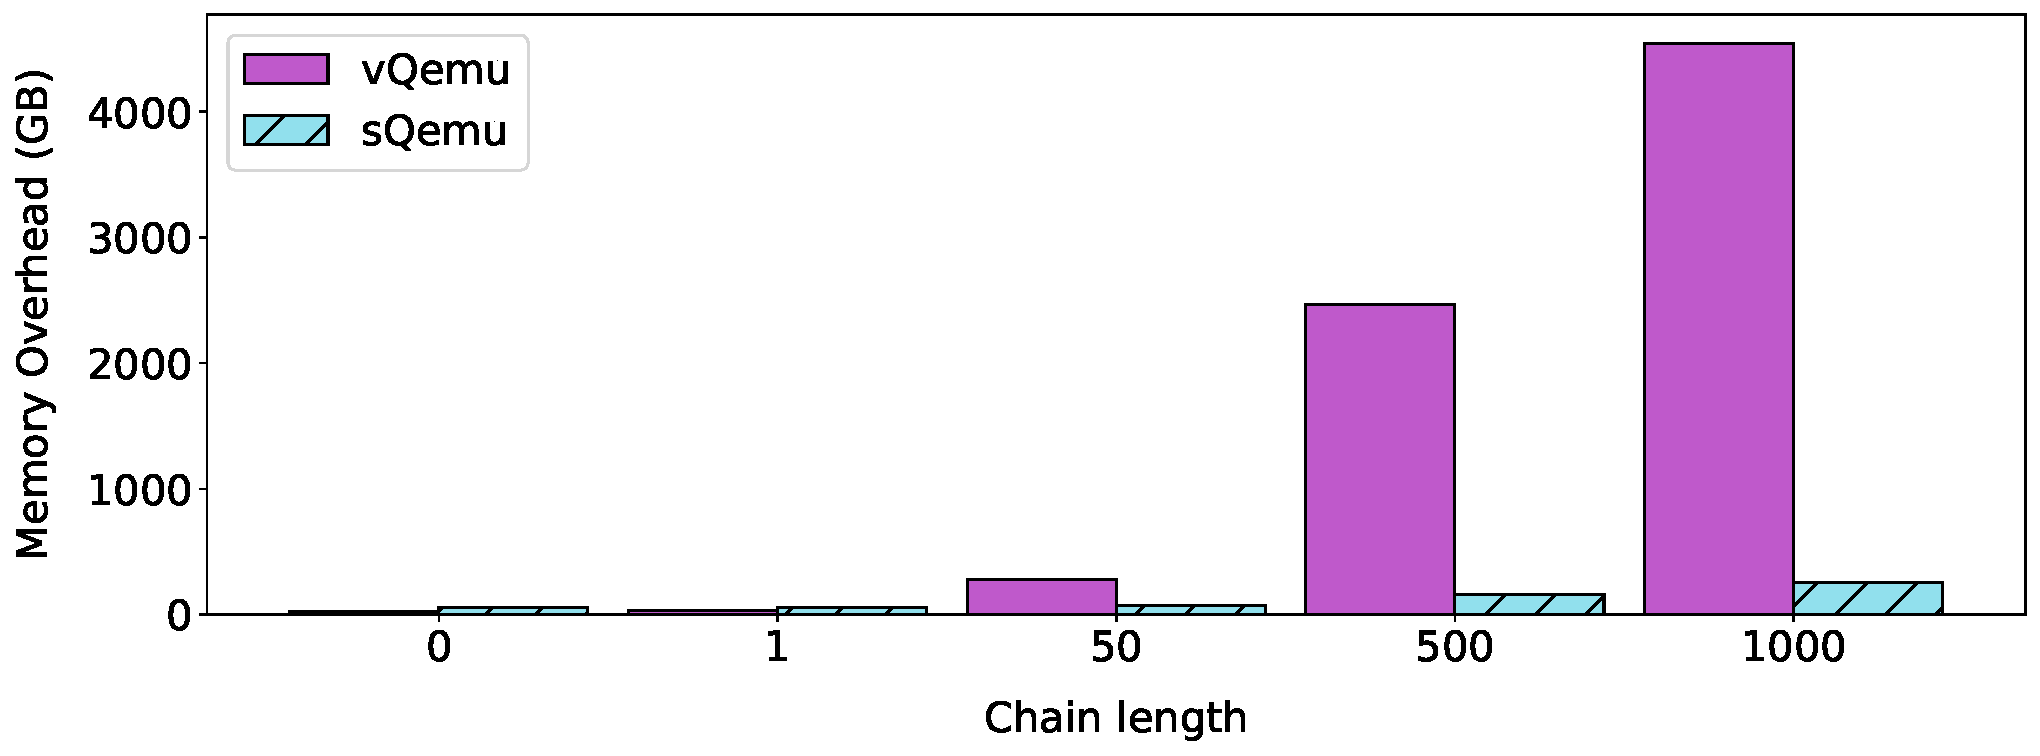
\includegraphics[width=0.45\textwidth]{memory_consumption.pdf}
		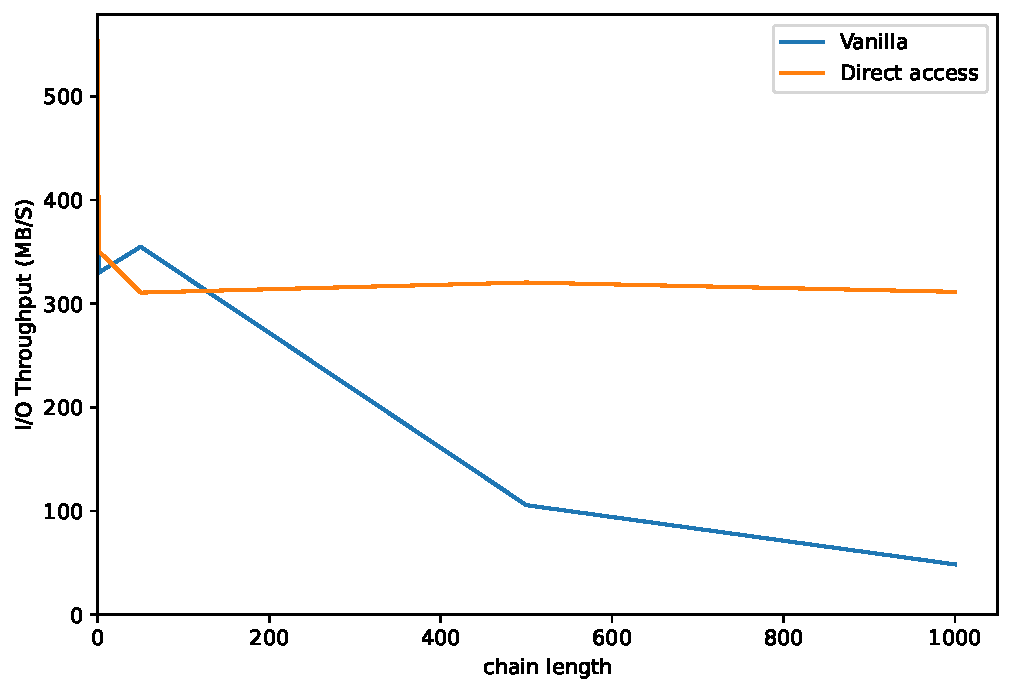
\includegraphics[width=0.45\textwidth]{workload_dd_throughput.pdf}
		\caption{Memory consumption and Throughput (I/O) during the workload}
		\label{fig:fig3}
	\end{figure}
	
	\section*{Startup duration}
	This section evaluates the startup duration of a VM for both vanilla and direct-access.
	%The first evaluation i did, presenting the startup duration of a Virtual machine, comparison between our version and vanilla qemu
	
	\begin{figure}[h]
		\center
		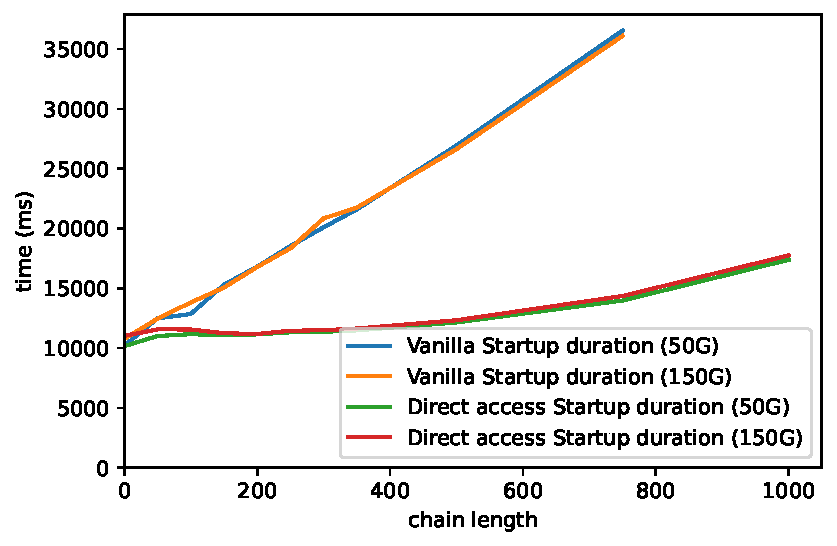
\includegraphics[width=0.45\textwidth]{startup_duration.pdf}
		\caption{Startup, vanilla and direct-access version on 50G and 150G disk}
		\label{fig:fig34}
	\end{figure}

	\section*{Cache \emph{hit} and \emph{missed} treatment times}
	
	% It is important to notice we are always working on chain of snapshots. 
	% Here, we call \textit{Cache hit}, all the operations needed by the driver to get access successfully to an l2 entry describing a cluster without going on image file to find it (i.e looking only in memory). 
	% And then, \textit{Cache Missed} is when we had to go at least once on image files (important to precise we can go many times on disk to look in the different snapshots image file). 
	\stella{il faut expliquer tout ce qui précédait là (la diff entre hit et miss) dans la section où tu parles des events en reformulant mieux}
	We perfom this experiment on an HDD hard disk (as used by most of cloud providers), and an SSD hard disk, supposing that we are in the best cases of hard disk speed.
	
	\subsection*{Cache Missed treatment times}
	
	\textit{Van/Dir x: Vanilla/Direct-access run on a chain of x snapshots. \textbf{base} for a chain without snapshots. \stella{ici tu parles de base alors que dans une figure précédente tu as utilisé 0 pr parler d'image sans snap il faut uniformiser cela}}
	\begin{figure}[h]
		\center
		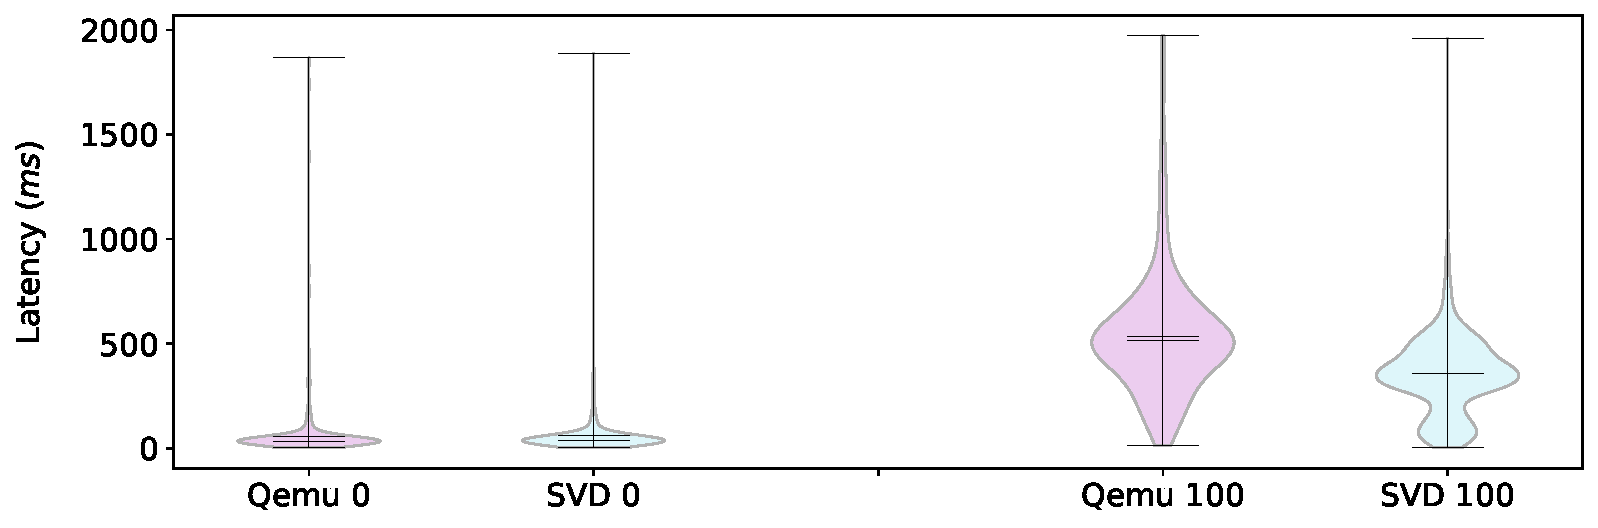
\includegraphics[width=0.45\textwidth]{MISSED_time_hdd.pdf}
		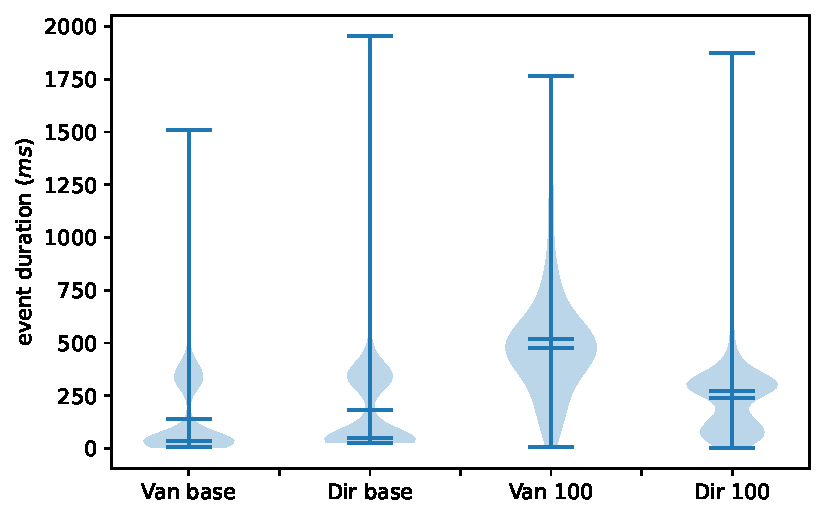
\includegraphics[width=0.45\textwidth]{MISSED_time_ssd.pdf}
		\caption{On the left, boxplot presenting time to resolve cache missed with images file stored on a HDD hard disk. On the right, the same with images file on an SSD hard disk}
		\label{fig:fig-a}
	\end{figure}

	We can make the following observations.
	(1) Obviously, when there is no snapshot, there are no differences between the 2 versions and times of treatment are the same.
	(2) When the chain length increases, treatment of a cache missed takes generally about $500 ms$ with vanilla against less than $300 ms$ with direct-access, for a chain of 100 snapshots.
	\stell{essaie de mieux expliquer le paragraphe suivant je ne comprends pas: est ce un plus pour le travail de le soulever ? (vu que tu as dit que c'était pas notre but): si oui mieux formuler, sinon l'omettre}
	% Another notice we did was the large repartition of time in vanilla version. This large repartition of time report another problem which is the unpredictability of performance, due to the time which can have a variety of values in this large field of possible values. Our solution try somehow to reduce this large repartition possibility but don't cancel it totally; but it is normal. It's not the goal of our work.
	
	\subsection*{Cache hit times}
	
	\begin{figure}[h]
		\center
		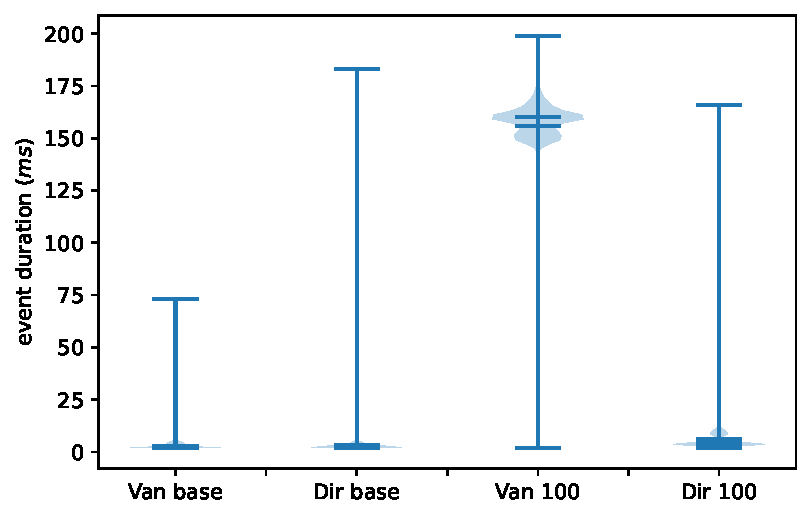
\includegraphics[width=0.45\textwidth]{HIT_time_hdd.pdf}
		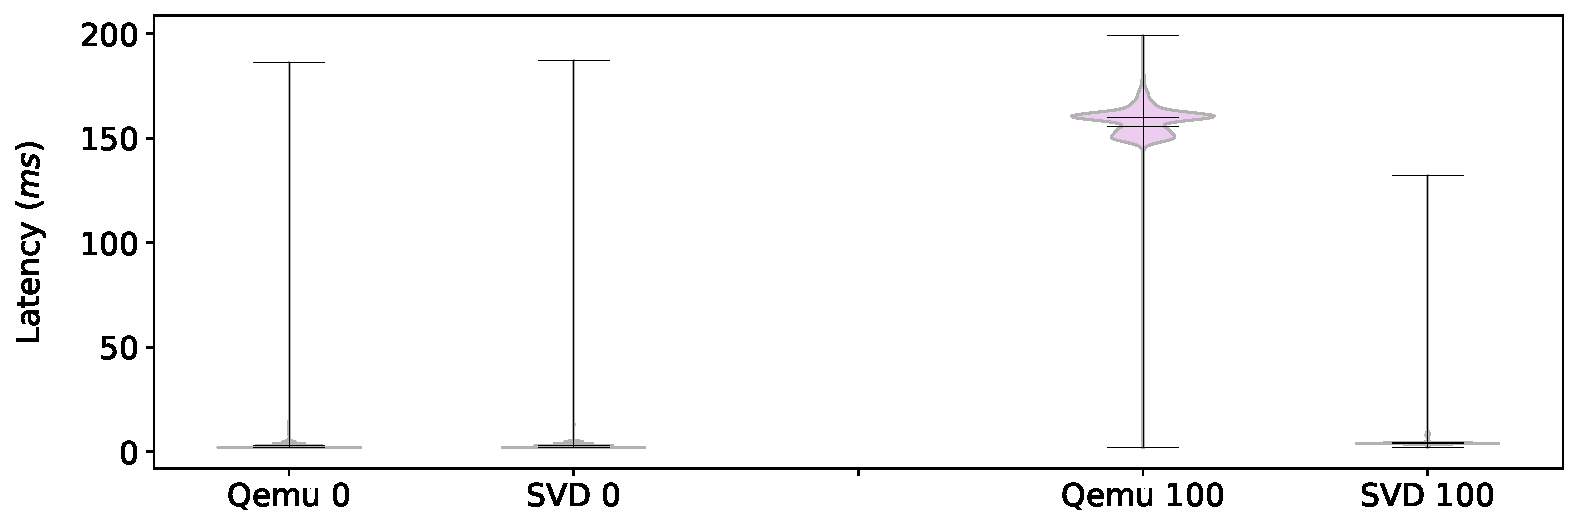
\includegraphics[width=0.45\textwidth]{HIT_time_ssd.pdf}
		\caption{On the left, boxplot presenting time to get value in the cache with images file stored on a HDD hard disk. On the right, the same with images file on an SSD hard disk}
		\label{fig:fig_b}
	\end{figure}

	A hit time is not affected by the type of the disk (HDD or SSD) as it is done in-memory.
	Hits are often short events in general (at the order of $\mu s$). 
	But when scaling by using a chain of 100 snapshots for example, vanilla takes much longer time because each hit knocks on all the intermediate cache levels.
	With direct-access, a hit only knocks on the target cache level. 
	This is why regardless the number of snapshots, the time of a hit event with direct-access is almost the same.

	% Nothing to say about chain of 0 snapshot. Hits are often few operations at the order of $\mu$s. So it's normal that times are so small here, either on HDD or SSD hard disk.
	% But, when we scale, by using chain of 100 snapshots for example, in vanilla we take too much time because each hit operation knock on all the intermediate caches where in our solution, we only knock on the first cache and the one where the information we are looking is. It is why our times are near the times observed as if there are no snapshots.
	% The other notice we can do is that hit times are not affect by the type of hard disk used (HDD/SDD) because all hits are done in memory.

	\section*{Performance evaluation}
	
	We vary the cache size of the VM while starting it and launch a random workload (e.g., fio).
	The goal is to compare both solution when using the same amount of cache. 
	
	\begin{figure}[h]
		\center
		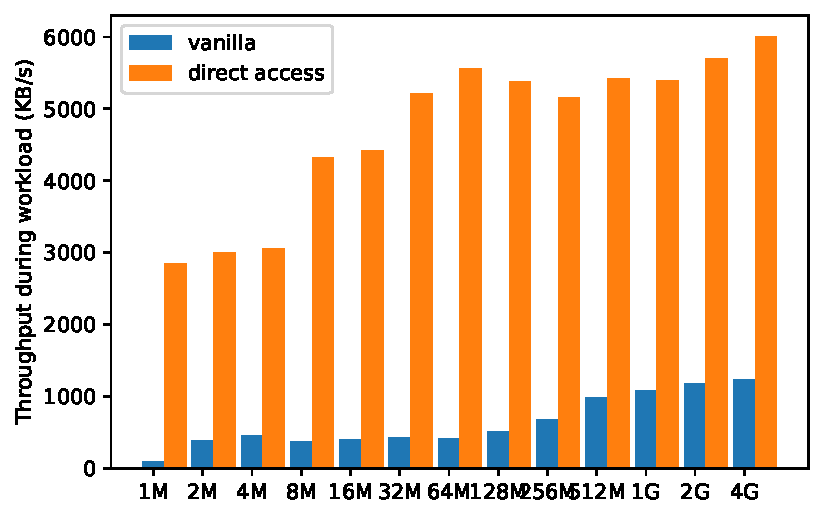
\includegraphics[width=0.45\textwidth]{cache_variation.pdf}
		\caption{Cache variation while running a random read workload on a chain of 500 snapshots}
		\label{fig:fig-c}
	\end{figure}

	% Nothing to say here too i guess, our solution is always better; even when the performance of vanilla increases with cache allocated to him that increased, our solution is always better.
	We observe that direct-access always has a better throughput compared to vanilla.
	And when the cache size becomes greater than 4 MB, direct-access performance becomes almost constant. 
	This is due to the fact that 4 MB is the minimal cache size required by direct-access for disk size and the chain length \stella{il faut dire à l'intro de la section où tu décris l'expériment}.
	
	\section*{Cache deduplication in vanilla}
	This experiment demontrates the cache deduplication with vanilla.
	We count for each snapshot, the cluster metadata that are present in the cache and compute the amount of waste memory. \stell{explique ici ce que tu entends par "perte", j'imagine que c'est le fait que ce soit répliqué alors que ce n'est pas nécessaire}
	The experiment is done with a chain of 100 snapshots and minimal cache size required is 7 MB.
	% In order to prove that really exists cache deduplication in vanilla, we did this other evaluation: Counting cluster metadata that were presented many times in the differents cache of each snapshot; then calculate the amount of memory we wasted. The evaluation was did on a chain of 100 snapshots, The cache memory needed to contain all the metadata is 7MB in this case.
	Fig.~\ref{xxx} presents the memory wasted (duplication) for fio (random read) workload from the entire VM life.
	
	\begin{figure}[h]
		\center
		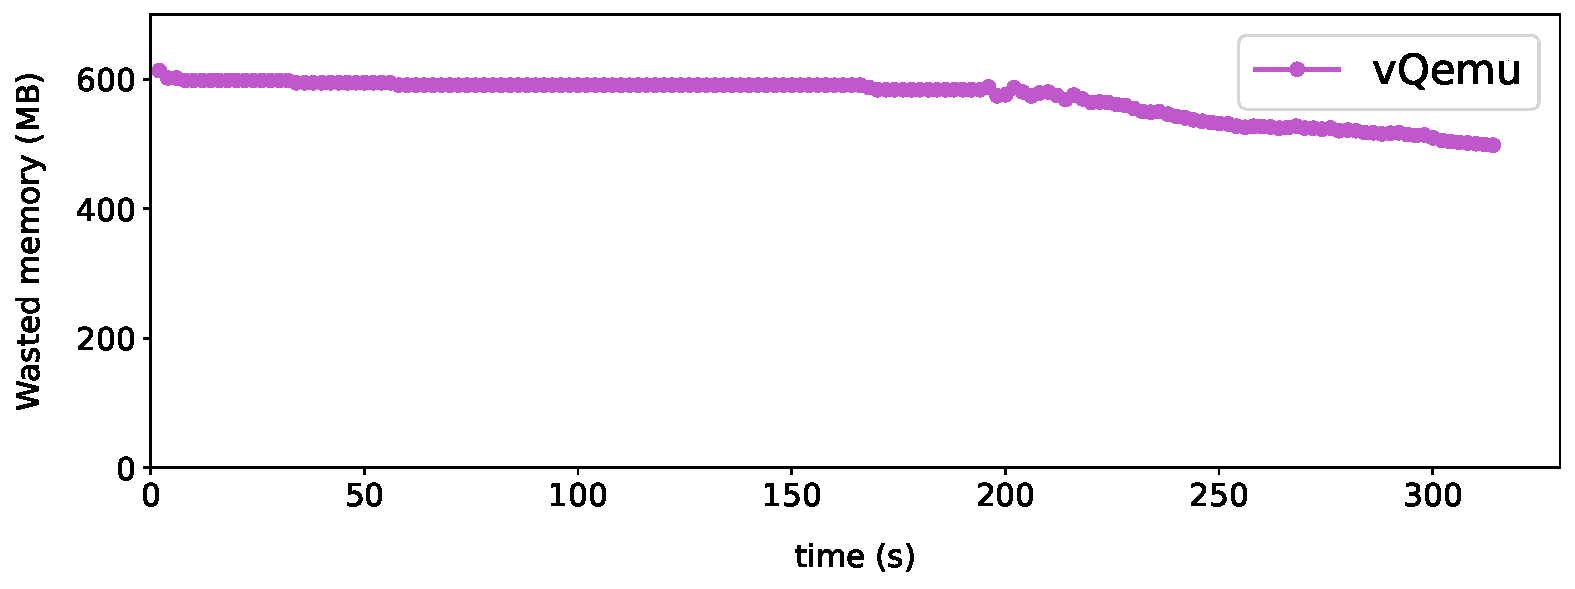
\includegraphics[width=0.45\textwidth]{dupli_memory.pdf}
		\caption{Startup, vanilla and direct-access version on 50G and 150G disk}
		\label{fig:fig-d}
	\end{figure}

\end{document}